\documentclass[journal]{IEEEtranTIE}
\usepackage{graphicx}
\usepackage[noadjust]{cite}
\usepackage{picinpar}
\usepackage{amsmath}
\usepackage{stfloats}
%%\usepackage{dblfloatfix}
\usepackage{url}
\usepackage{flushend}
\usepackage[latin1]{inputenc}
\usepackage{colortbl}
\usepackage{soul}
\usepackage{multirow}
\usepackage{pifont}
\usepackage{color}
\usepackage{alltt}
\usepackage[hidelinks]{hyperref}
\usepackage{enumerate}
\usepackage{siunitx}
\usepackage{breakurl}
\usepackage{epstopdf}
\usepackage{pbox}

%% My packages
%% \usepackage[cmex10]{amsmath}
%% \interdisplaylinepenalty=2500
\usepackage{algpseudocode}
%% \usepackage{array}
\usepackage[caption=false,font=footnotesize]{subfig}

\usepackage{tikz}
\usetikzlibrary{external}
\usetikzlibrary{arrows.meta}
\tikzexternalize[prefix=./] %  activate
%% \usepackage{mathabx}


\newcommand{\hide}[1]{\ignorespaces}
\newcommand{\jx}[1]{{\bf Jiaxiang: }#1{ \bf End}}
\newtheorem{theorem}{Theorem}
\newtheorem{lemma}[theorem]{Lemma}
\newtheorem{definition}[theorem]{Definition}

% Define the fontsize in environment {verbatim}
\makeatletter
\def\verbatim{\small\@verbatim \frenchspacing\@vobeyspaces \@xverbatim}
%\def\verbatim@font{\small\ttfamily}
\makeatother

\usepackage{microtype}

\begin{document}

\tikzsetnextfilename{rms}
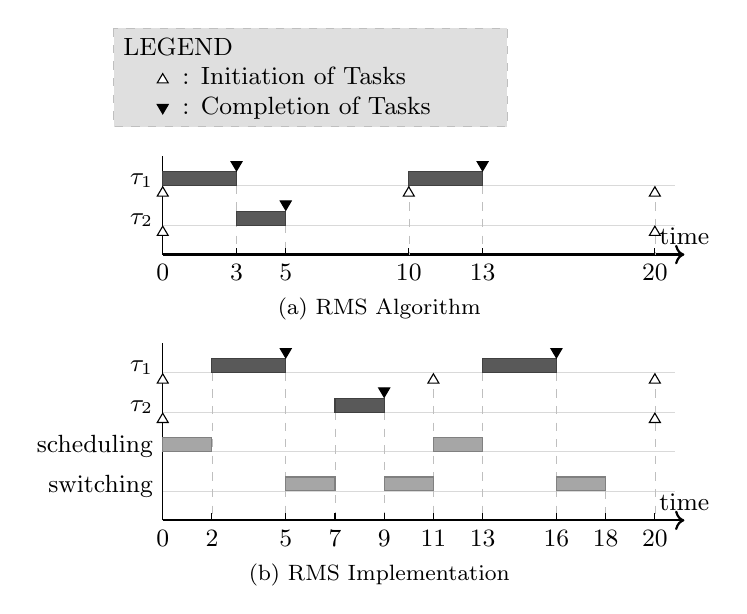
\begin{tikzpicture}[font=\small,scale=1.25,
    % styles
    system task/.style={fill=gray!70,draw=gray},
    periodic task/.style={fill=gray!70!black,draw=gray!50!black},
    task line/.style={gray!30,very thin},
    time line/.style={gray!50,very thin,dashed},
    short line/.style={gray!50,very thin,dashed},
    init/.style={{Triangle[fill=white,scale=1.1]}-},
    complete/.style={{Triangle[scale=1.1]}-}]

  % legend
  \begin{scope}[xshift=-2cm]  
    \draw [fill=gray!25,draw=gray!50,dashed] (1.5,2.3) rectangle +(4,-1);
    \draw (1.5,2.3) node [below right] {LEGEND};
    \draw [init] (2,1.85) -- +(0,-0.01);
    \draw (2.1,2) node [below right] {: Initiation of Tasks};
    \draw [complete] (2,1.42) -- +(0,0.1);
    \draw (2.1,1.7) node [below right] {: Completion of Tasks};
  \end{scope}

  %%% RMS Algorithm
  \begin{scope}
  
    % grid
    \foreach \x in {0.3,0.7}
      \draw[task line] (0,\x) -- (5.2,\x);

    % axes
    \draw[->,thick] (0,0) node [below] {$0$} -- (5.3,0) node [above] {time};
    \draw[thin] (0,0) -- (0,1);

    % time indicator
    \draw [time line] (0.75,0.7) -- (0.75,0);
    \draw (0.75,0) node [below] {$3$} -- +(0,2pt);
    \draw [time line] (1.25,0.3) -- (1.25,0);
    \draw (1.25,0) node [below] {$5$} -- +(0,2pt);
    \draw [time line] (2.5,0.7) -- (2.5,0);
    \draw (2.5,0) node [below] {$10$} -- +(0,2pt);
    \draw [time line] (3.25,0.7) -- (3.25,0);
    \draw (3.25,0) node [below] {$13$} -- +(0,2pt);

    \draw [time line] (5,0.7) -- (5,0);
    \draw (5,0) node [below] {$20$} -- +(0,2pt);
    
    % tasks
    \draw [periodic task] (0,0.7) rectangle +(0.75,0.14);
    \draw [periodic task] (0.75,0.3) rectangle +(0.5,0.14);
    \draw [periodic task] (2.5,0.7) rectangle +(0.75,0.14);

    % text
    \draw (0,0.75) node [left] {$\tau_1$};
    \draw (0,0.35) node [left] {$\tau_2$};
    \path (0,0.75) node [left,text opacity=0] {scheduling};
    \path (0,0.35) node [left,text opacity=0] {switching};    

    % initiation of tasks
    \foreach \x in {0,2.5,5}
      \draw [init] (\x,0.7) -- +(0,-0.01);
    \foreach \x in {0,5}
      \draw [init] (\x,0.3) -- +(0,-0.01);  

    % completion of tasks
    \draw [complete] (0.75,0.84) -- +(0,0.01);
    \draw [complete] (3.25,0.84) -- +(0,0.01);
    \draw [complete] (1.25,0.44) -- +(0,0.01);

    % label of subfigure
    \draw (2.2,-0.55) node [inner sep=0pt] {\footnotesize (a) RMS Algorithm};

  \end{scope}

  %%% RMS Implementation
  \begin{scope}[yshift=-2.7cm]

    % grid
    \foreach \x in {0.3,0.7,1.1,1.5}
      \draw[task line] (0,\x) -- (5.2,\x);

    % axes
    \draw[->,thick] (0,0) node [below] {$0$} -- (5.3,0) node [above] {time};
    \draw[thin] (0,0) -- (0,1.8);

    % time indicator
    \draw [time line] (0.5,1.5) -- (0.5,0);
    \draw (0.5,0) node [below] {$2$} -- +(0,2pt);
    \draw [time line] (1.25,1.5) -- (1.25,0);
    \draw (1.25,0) node [below] {$5$} -- +(0,2pt);
    \draw [time line] (1.75,1.1) -- (1.75,0);
    \draw (1.75,0) node [below] {$7$} -- +(0,2pt);
    \draw [time line] (2.25,1.1) -- (2.25,0);
    \draw (2.25,0) node [below] {$9$} -- +(0,2pt);
    \draw [time line] (2.75,1.5) -- (2.75,0);
    \draw (2.75,0) node [below] {$11$} -- +(0,2pt);
    \draw [time line] (3.25,1.5) -- (3.25,0);
    \draw (3.25,0) node [below] {$13$} -- +(0,2pt);
    \draw [time line] (4,1.5) -- (4,0);
    \draw (4,0) node [below] {$16$} -- +(0,2pt);
    \draw [time line] (4.5,0.3) -- (4.5,0);
    \draw (4.5,0) -- +(0,2pt);
    \draw (4.5,0) node [below] {$18$};
    \draw [time line] (5,1.5) -- (5,0);
    \draw (5,0) node [below] {$20$} -- +(0,2pt);
    
    % tasks
    \draw [system task] (0,0.7) rectangle +(0.5,0.14);
    \draw [periodic task] (0.5,1.5) rectangle +(0.75,0.14);
    \draw [system task] (1.25,0.3) rectangle +(0.5,0.14);
    \draw [periodic task] (1.75,1.1) rectangle +(0.5,0.14);
    \draw [system task] (2.25,0.3) rectangle +(0.5,0.14);
    \draw [system task] (2.75,0.7) rectangle +(0.5,0.14);
    \draw [periodic task] (3.25,1.5) rectangle +(0.75,0.14);
    \draw [system task] (4,0.3) rectangle +(0.5,0.14);

    % text
    \draw (0,1.55) node [left] {$\tau_1$};
    \draw (0,1.15) node [left] {$\tau_2$};
    \draw (0,0.75) node [left] {scheduling};
    \draw (0,0.35) node [left] {switching};    

    % initiation of tasks
    \foreach \x in {0,2.75,5}
      \draw [init] (\x,1.5) -- +(0,-0.01);
    \foreach \x in {0,5}
      \draw [init] (\x,1.1) -- +(0,-0.01);  

    % completion of tasks
    \draw [complete] (1.25,1.64) -- +(0,0.01);
    \draw [complete] (2.25,1.24) -- +(0,0.01);
    \draw [complete] (4,1.64) -- +(0,0.01);
    
    % label of subfigure
    \draw (2.2,-0.55) node [inner sep=0pt] {\footnotesize (b) RMS Implementation};
  \end{scope}
\end{tikzpicture}


\end{document}
